\chapter{实例学习:Tkinter}

\section{GUI}

我们迄今为止编写的程序都是字符界面下的,现在很多程序使用
图形用户接口(graphical user interfaces},简称{\bf GUIs}。

\index{GUI}
\index{graphical user interface 图形用户接口}
\index{Tkinter}

Python提供了多种选择来来编写GUI程序,包括wxPython, Tkinter和
Qt\footnote{译注:还有一个非常流行的就是pyGtk}。每种框架都优缺参半。
这也就是为什么Python在图形库上没有形成一个标准的原因。

这一章,我要讲述的是Tkinter,因为我认为它是最容易入手的。本章的很多概念同样适用于其他GUI模块。

有一些关于Tkinter的书和网站。网上最好的资料是Fredrik Lundh写的{\em An Introduction to Tkinter}。

\index{Gui module}
\index{module!Gui}
\index{Swampy}

我也写了一个模块{\tt Gui.py},包含在Swampy里。它提供了Tkinter里函数和
类的简单接口。这章的例子就是以这个模块为基础。

下面是一个创建显示Gui的简单例子:

要创建一个GUI,必须导入{\tt Gui}模块,并且实例化一个Gui对象:

\beforeverb
\begin{verbatim}
from Gui import *

g = Gui()
g.title('Gui')
g.mainloop()
\end{verbatim}
\afterverb
%

当运行这段代码,会出现一个窗口,窗口由灰色的区域和标题{\sf Gui}组成。
{\tt mainloop}运行事件循环,等待用户操作,然后做出相应的反应。这是一个无限循环,一直运行到用户关闭窗口,或者按下Control-C,或者其他能使程序终止的操作。

\index{event loop 事件循环}
\index{loop!event}
\index{infinite loop 无限循环}
\index{loop!infinite}

这个Gui没有做什么事情,因为它没有任何的控件。控件是构成GUI的元素,
包括:

\index{widget 控件}

\begin{description}

\item [Button 按钮:]包含文本或图像的控件,当被按压时,产生一个动作。

\item [Canvas 画布:]能够显示直线,矩形,圆和其他图形的区域。

\item [Entry 输入框:]用户可以输入文本的区域。

\item [Scrollbar 滚动条:] 控制其他空间可见部分的空间。

\item [Frame 框:]容纳其他控件的容器,通常是不可见的。

\end{description}

创建Gui时的空白灰色区域就是一个框。当新建一个控件,就会被加到这个框。

\section{按钮和回调}

\index{Button widget 按钮控件}
\index{widget!Button}

{\tt bu}方法创建一个按钮空间:

\beforeverb
\begin{verbatim}
button = g.bu(text='Press me.')
\end{verbatim}
\afterverb

{\tt bu}方法的返回值是按钮对象。框里的按钮是这个对象的图形化显示;
可以通过调用按钮的方法控制按钮。

\index{option}

{\tt bu}可以通过32个参数控制按钮的外形和功能,这些参数叫做选项。除了
提供全部的32个选项,你可以提供关键的参数,像\verb"text='Press me.'",
指定你需要的选项即可,其他的使用缺省值。

\index{keyword argument 关键参数}
\index{argument!keyword}

当向一个框添加控件时,框就变被”收缩包裹“了,也就是框收缩成按钮般大小。
如果想添加更多的空间,框自动增长来安排他们。

\index{Label widget}
\index{widget!Label}

{\tt la}方法创建标签控件:

\beforeverb
\begin{verbatim}
label = g.la(text='Press the button.')
\end{verbatim}
\afterverb

缺省情况下,Tkinter从上至下安排空间,然后使其居中。我们不久将会看到如何覆盖这种行为。

如果按下按钮,你会看到它也没有做什么事情。那是因为你还没有“启动”它,也就是说,你还没有告诉它做什么!

控制一个按钮行为的选项是{\tt command}。{\tt command}的值是一个函数,它在按钮按下的时候执行。比如,下面是一个函数创建一个新的标签:

\beforeverb
\begin{verbatim}
def make_label():
    g.la(text='Thank you.')
\end{verbatim}
\afterverb

现在我们可以创建一个按钮,把这个函数作为{\tt command}:

\beforeverb
\begin{verbatim}
button2 = g.bu(text='No, press me!', command=make_label)
\end{verbatim}
\afterverb

当按下这个按钮,程序执行\verb"make_label",一个新的标签就会出现。

\index{callback 回调}

{\tt command}的值是一个函数对象,也叫回调函数,因为当你调用{\tt bu}
创建一个按钮,用户按下按钮时,执行流回调了。

\index{event-driven programming 时间驱动编程}

这种控制流是事件驱动编程的特点。用户动作,像按下按钮和击键,叫做事件
。在事件驱动编程中,执行流是由用户动作控制而不是程序员。

事件驱动编程的最大挑战在于为任何的用户动作建立一系列的控件及回调函数(至少更产生适当的错误信息)。

\begin{ex}
编写一个程序,创建只有一个按钮的GUI。当按钮被按下时,程序创建第二个按钮。当第二个按钮被按下时,应该创建一个标签,显示"Nice job!"。

如果按了多次按钮,会出现什么情况?

可以参看我的解答\url{thinkpython.com/code/button_demo.py}

\end{ex}


\section{画布控件}

\index{Canvas widget 画布控件}
\index{widget!Canvas}

画布是用途最多的空间之一,创建一个可以绘制直线,圆,和其他形状的区域。如果你做了练习\ref{画布},你已经熟悉了画布。

{\tt ca}创建了一个新的画布:

\beforeverb
\begin{verbatim}
canvas = g.ca(width=500, height=500)
\end{verbatim}
\afterverb

{\tt width}和{\tt height}是用像素表示的画布尺度。

\index{config method}
\index{method!config}

在创建了一个控件之后,仍然可以通过{\tt config}方法来修改选项的值。比如,{\tt bg}选项改变背景颜色:

\beforeverb
\begin{verbatim}
canvas.config(bg='white')
\end{verbatim}
\afterverb

{\tt bg}的值是颜色名。不同的Python拥有不同的合法颜色名,但是所有的
python实现都会提供至少如下的颜色名:

\begin{verbatim}
white   black
red     green    blue   
cyan    yellow   magenta
\end{verbatim}
\afterverb
%

画布上的图形叫做项。比如,画布方法{\tt circle}绘制(你猜是这样)一个圆:

\index{Canvas item 画布项}
\index{item!Canvas}

\beforeverb
\begin{verbatim}
item = canvas.circle([0,0], 100, fill='red')
\end{verbatim}
\afterverb


第一个参数是一个坐标对,指明了圆心的位置;第二个是半径。

\index{Canvas coordinate 画布坐标}
\index{coordinate!Canvas}

{\tt Gui.py}提供了一个标准的笛卡尔坐标系,原点在画布的中央,$y$正
半轴向上。这个其他的图像系统不一样,他们的原点在左上角,$y$正半轴向下。

{\tt fill}选项指明圆应该用红色来填充。

{\tt circle}的返回值是一个项对象,提供了修改画布上项的方法。蔽日,
可以使用{\tt config}改变圆的任意一个选项:

\beforeverb
\begin{verbatim}
item.config(fill='yellow', outline='orange', width=10)
\end{verbatim}
\afterverb

{\tt width}是用像素表示的轮廓厚度;{\tt outline}是颜色。

\begin{ex}
\label{circle}

编写一个程序创建一个画布和按钮。当用户按下按钮,应该在华布上画一个圆。
\end{ex}

\section{坐标序列}

\index{coordinate sequence 坐标序列}
\index{sequence!coordinate}

{\tt rectangle}方法接受坐标序列指明对顶角的位置。下面这个例子
绘制了一个绿色的矩形,坐下角在原点,右上角在$(200,100)$:

\beforeverb
\begin{verbatim}
canvas.rectangle([[0, 0], [200, 100]], 
                 fill='blue', outline='orange', width=10)
\end{verbatim}
\afterverb

这种指定角的方法叫做界定盒子,因为,两个点界定了一个矩形。

\index{bouding box}

{\tt oval}接受一个界定的盒子,在矩形里绘制一个椭圆。

\beforeverb
\begin{verbatim}
canvas.oval([[0, 0], [200, 100]], outline='orange', width=10)
\end{verbatim}
\afterverb

{\tt line}接受坐标序列,绘制线段连接各个点。下面这个例子绘制了三角形的两个边:

\beforeverb
\begin{verbatim}
canvas.line([[0, 100], [100, 200], [200, 100]], width=10)
\end{verbatim}
\afterverb

{\tt polygon}接受同样的参数,但是它绘制了最后一条边(如果有必要),并且
填充它:

\beforeverb
\begin{verbatim}
canvas.polygon([[0, 100], [100, 200], [200, 100]],
               fill='red', outline='orange', width=10)
\end{verbatim}
\afterverb

\section{更多的控件}

\index{Text widget 文本空间}
\index{widget!Text}

Tkinter提供了两个控件让用户输入文本:一个输入框,只能单行输入,和
文本控件,可以输入多行。

\index{Entry widget 输入框}
\index{widget!Entry}

{\tt en}创建一个输入框:

\beforeverb
\begin{verbatim}
entry = g.en(text='Default text.')
\end{verbatim}
\afterverb

{\tt text}选项允许你在输入框创建时把文本放进输入框。{\tt get}方法
返回文本框的内容(可能被用户改变了):

\beforeverb
\begin{verbatim}
>>> entry.get()
'Default text.'
\end{verbatim}
\afterverb

{\tt te}创建一个文本控件:

\beforeverb
\begin{verbatim}
text = g.te(width=100, height=5)
\end{verbatim}
\afterverb
%

{\tt width}和{\tt height}是空间中字符数和行数的大小。

{\tt insert}把文本插入文本控件:

\beforeverb
\begin{verbatim}
text.insert(END, 'A line of text.')
\end{verbatim}
\afterverb
%

{\tt END}是一个特别的索引,代表文本框里的最后一个字符。

你可以指定用点索引(dotted index来插入字符,像{\tt 1.1},小数点前面
的数字代表行数,后面的代表列数。下面的例子把\verb"'nother'"加到第一行第一个字符之后。

\beforeverb
\begin{verbatim}
>>> text.insert(1.1, 'nother')
\end{verbatim}
\afterverb

{\tt get}方法从文本控件读取文本;接受起始索引作为参数。下面的例子返回文本控件的所有内容,包括换行符:

\beforeverb
\begin{verbatim}
>>> text.get(0.0, END)
'Another line of text.\n'
\end{verbatim}
\afterverb
%

{\tt delete}方法从文本控件里移除文本;下面的例子删除除了开头的两个字符:

\beforeverb
\begin{verbatim}
>>> text.delete(1.2, END)
>>> text.get(0.0, END)
'An\n'
\end{verbatim}
\afterverb
%

\begin{ex}
\label{circle2}

修改练习\ref{circle}的解答,增加一个输入框和按钮。当用户按下新增加的
按钮时,程序从输入框读取一个颜色名,用它改变圆的填充色。用{\tt config}修改圆,不要新建一个圆。

你的程序应该能处理没有无颜色名或者颜色名不合法的情况。

参看我的解答\url{thinkpython.com/code/circle_demo.py}.

\end{ex}

\section{排列控件}

迄今,我们只是上下安排控件,但是大多数的GUIs的布局都是很复杂的。比如,下面是一个稍微有点复杂的TurtleWorld(参看\ref{turtlechap}章节)。

\beforefig
\centerline{
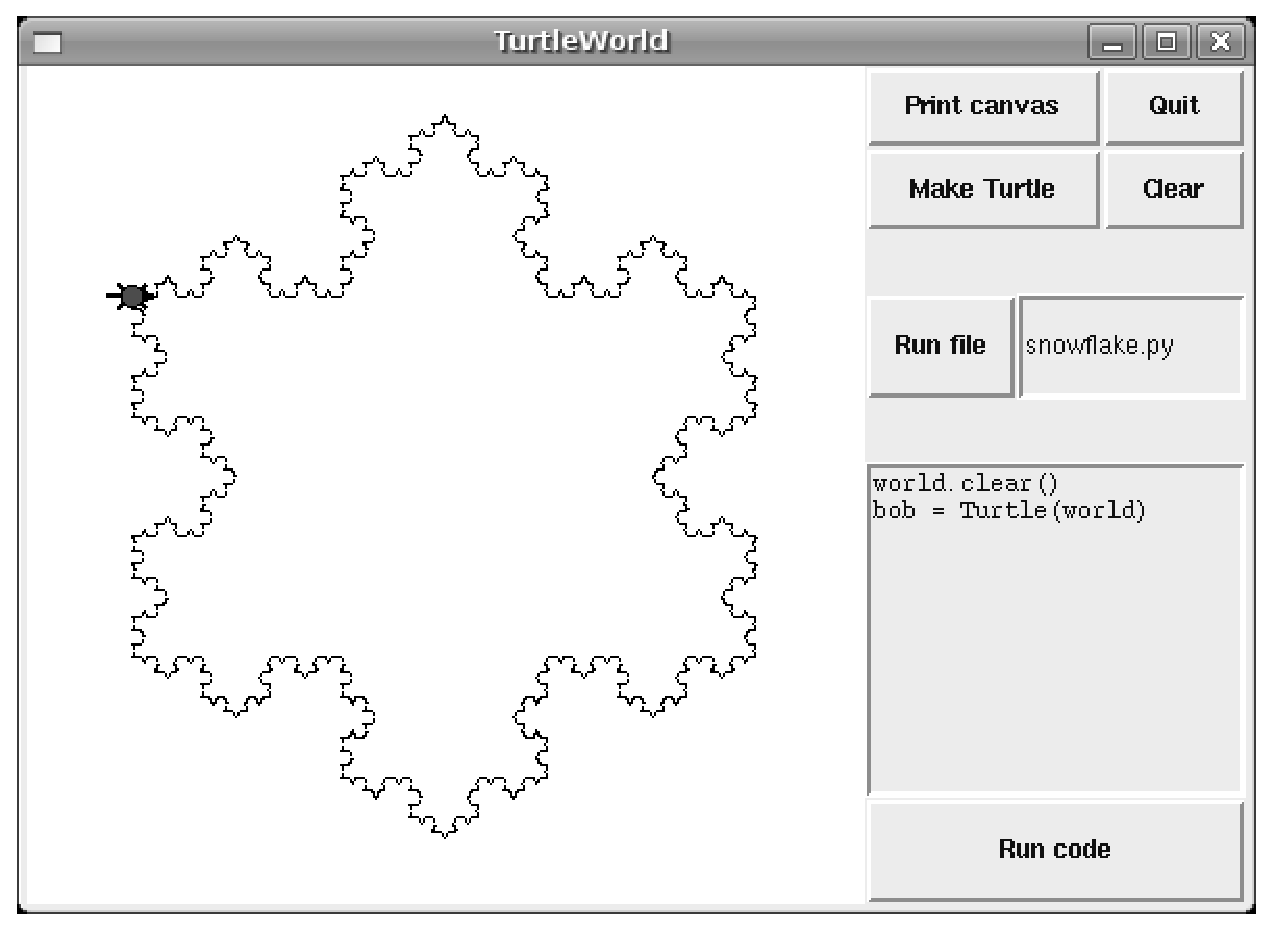
\includegraphics[width=1.0\textwidth]{figs/TurtleWorld.eps}
}
\afterfig


这个部分给出了创建这个GUI的代码,分解成一系列的步骤。可以下载完整的程序 \url{thinkpython.com/code/SimpleTurtleWorld.py}。

在顶级,这个GUI包含了两个控件---一个画布和一个框---并行排列着。所以第一步是创建行。

\index{SimpleTurtleWorld class}
\index{class!SimpleTurtleWorld}

\beforeverb
\begin{verbatim}
class SimpleTurtleWorld(TurtleWorld):
    """This class is identical to TurtleWorld, but the code that
    lays out the GUI is simplified for explanatory purposes."""

    def setup(self):
        self.row()
        ...
\end{verbatim}
\afterverb
%

{\tt setup}是创建并布局控件的函数。布局控件叫做包装。

\index{packing widgets 包装控件}
\index{widget,packing}
\index{Frame widget}
\index{widget!Frame}

{\tt row}行创建了一个行框,使它成为当前框。知道这个框被关闭或者新的框被船舰,所有后创建的控件都被包装在这行里。

下面是创建画布和列框,容纳其他控件的代码:

\beforeverb
\begin{verbatim}
        self.canvas = self.ca(width=400, height=400, bg='white')
        self.col()
\end{verbatim}
\afterverb
%

列框里的第一个控件是格子框,它包含了四个两两相邻的按钮。

\beforeverb
\begin{verbatim}
        self.gr(cols=2)
        self.bu(text='Print canvas', command=self.canvas.dump)
        self.bu(text='Quit', command=self.quit)
        self.bu(text='Make Turtle', command=self.make_turtle)
        self.bu(text='Clear', command=self.clear)
        self.endgr()
\end{verbatim}
\afterverb
%

{\tt gr}创建网格;参数是列的数目。网格里的控件是按照从左至右,从上到下安排的。

\index{callback 回调}
\index{bound method  绑定方法}
\index{method, bound}
\index{subject 主体}

第一个按钮使用{\tt self.canvas.dump}作为回调函数;第二个使用{\tt self.quit}。有三种绑定方法(bound methods),意味着他们和一个特定的对象绑定在一起。当他们被调用,他们是作用在该对象上。

列的下一个控件是行框,包含了一个按钮和输入框。

\beforeverb
\begin{verbatim}
        self.row([0,1], pady=30)
        self.bu(text='Run file', command=self.run_file)
        self.en_file = self.en(text='snowflake.py', width=5)
        self.endrow()
\end{verbatim}
\afterverb

{\tt row}的第一个参数是引力列表,决定了控件之间多余的空间如何分配。
{\tt [0,1]}表明所有的空间都分配给第二个控件,这里是输入框。如果你
运行这段代码,改变窗口大小,将会看到输入框变大而按钮不变。

选项{\tt pady}在$y$轴方向填充,上下分别增加30像素的空间。

{\tt endrow}结束添加控件,所以以后创建的可空间会被包装在列框。{\tt Gui.py}保存了框的栈:

\begin{itemize}

\item 当使用{\tt row},{\tt col},或者{\tt gr}创建一个框,程序进入栈顶,并且变为当前框。

\item 当使用{\tt endrow},{\tt endcol}或{\tt endgr}来关闭一个框,程序弹出栈顶,把前一个框置为当前框。

\end{itemize}

\verb"run_file"方法读取输入框的内容,把它作为文件名,读取文件,
传递给\verb"run_code"。{\tt self.inter}是一个解释器对象,能够接受一个字符串,并且把它作为Python代码执行。

\beforeverb
\begin{verbatim}
    def run_file(self):
        filename = self.en_file.get()
        fp = open(filename)
        source = fp.read()
        self.inter.run_code(source, filename)
\end{verbatim}
\afterverb
%

最后两个控件是文本控件和按钮:

\beforeverb
\begin{verbatim}
        self.te_code = self.te(width=25, height=10)
        self.te_code.insert(END, 'world.clear()\n')
        self.te_code.insert(END, 'bob = Turtle(world)\n')

        self.bu(text='Run code', command=self.run_text)
\end{verbatim}
\afterverb
%

\verb"run_text"和\verb"run_file"相似,除了它从文本控件接受代码,
而不是从文件:

\beforeverb
\begin{verbatim}
    def run_text(self):
        source = self.te_code.get(1.0, END)
        self.inter.run_code(source, '<user-provided code>')
\end{verbatim}
\afterverb

不幸的是,控件布局的方式和其他语言是有差异的,甚至在Python的不同模块里也是有差异的。Tkinter自己也提供了3种不同的布局控件的方式。这些方法叫做几何管理器。这部分我演示的是“grid"几何管理器;其他的两种叫做"组装“和”放置“。

\index{geometry manager 几何管理器}

幸运的是,这部分的大多数概念对其他的GUI模块和其他语言也是适用的。

\section{菜单和可召唤的}

\index{Menubutton widget 菜单按钮}
\index{widget!Menubutton}

菜单按钮是一个看起来像按钮的控件,但是当按下它时,它弹出菜单。用户选择一个项以后,菜单消失。

下面是创建一个颜色选择菜单按钮的代米(可以从这个下载\url{thinkpython.com/code/menubutton_demo.py})):

\beforeverb
\begin{verbatim}
g = Gui()
g.la('Select a color:')
colors = ['red', 'green', 'blue']
mb = g.mb(text=colors[0])
\end{verbatim}
\afterverb
%

{\tt mb}创建一个菜单按钮。开始,按钮上的文本是缺省颜色名。下面的循环为每个颜色创建了一个菜单项:

\beforeverb
\begin{verbatim}
for color in colors:
    g.mi(mb, text=color, command=Callable(set_color, color))
\end{verbatim}
\afterverb

{\tt mi}的第一个参数是联系这些项在一起的菜单按钮。

\index{callback 回调}
\index{callable object 可调用对象}
\index{object!Callable}

{\tt command}选项是可调用对象,这个是个新内容。迄今为止,我们已经看到函数和绑定方法作为回调函数,如果不需要传递参数给函数,这个工作的很好。否则,你必须创建一个包含函数(像\verb"set_color")及其参数(像{\tt color})的可调用对象。


可调用对象存储了函数的引用和参数作为属性。然后,当用户点击菜单项的时候,回调函数调用函数并且传递存储的参数。

下面是\verb"set_color"函数:

\beforeverb
\begin{verbatim}
def set_color(color):
    mb.config(text=color)
    print color
\end{verbatim}
\afterverb
%

当用户选择一个菜单项时,\verb"set_color"被调用,它重新配置了菜单按钮显示新选择的颜色,同时也打印了颜色。如果你试着运行这个例子,你可以
确定当你选择一个项时\verb"set_color"被调用,当创建可调用对象时没有被调用。

\section{Binding 绑定}

\index{binding 绑定}
\index{callback 回调}

绑定就是控件,事件和回调函数之间的联系:当一个事件(像按下按钮)在一个控件上发生时,回调函数被调用。

很多控件都有缺省的绑定。比如,当你按下按钮,缺省的绑定改变了按钮的样子,看起来像被压平了一样。当释放按钮,绑定恢复了按钮的样子,然后调用
回调函数(由{\tt command}选项指定)


可以使用{\tt bind}方法覆盖缺省的帮定,或者增加一个新的绑定。比如,下面的
代码为画布创建了一个新的绑定(可以从这儿下载\url{thinkpython.com/code/draggable_demo.py})):

\beforeverb
\begin{verbatim}
ca.bind('<ButtonPress-1>', make_circle)
\end{verbatim}
\afterverb
%

第一个参数是一个事件字符串;这个事件在用户按下鼠标的左键时,发出。其他的鼠标事件包括 {\tt ButtonMotion}, {\tt ButtonRelease}和 
{\tt Double-Button}.


\index{event string 事件字符串}
\index{event handler 事件处理}

第二个参数是事件处理器。事件处理器是一个函数或者绑定方法,像回调函数一样,但是有一个重要的不同就是事件处理器接受一个事件对象作为参数。下面是一个例子:

\beforeverb
\begin{verbatim}
def make_circle(event):
    pos = ca.canvas_coords([event.x, event.y])
    item = ca.circle(pos, 5, fill='red')
\end{verbatim}
\afterverb

事件对象包含了事件类型和一些细节等信息,像鼠标指针的坐标。这个例子中
我们需要的信息是鼠标点击的位置。这些值都是以像素坐标保存的,由底层的图像系统定义。\verb"canvas_coords"方法把他们转换成"Canvas coordinates",这个值才能在画布方法中使用,像{\tt circle}。

\index{Event object}
\index{object!Event}

对于输入框来是哦,绑定\verb"<Return>"事件是很常见的,当用户按下{\sf Return}键时,就会发射。比如,下面的例子创建了一个按钮和输入框:

\beforeverb
\begin{verbatim}
bu = g.bu('Make text item:', make_text)
en = g.en()
en.bind('<Return>', make_text)
\end{verbatim}
\afterverb
%

用户在输入框里输入时,当按下按钮或者用户敲击{\sf Return}\verb"make_text"就被调用。为了使这个能公正常工作,我们需要一个能够被调用的函数作为
{\tt command}(无参数)或者作为事件处理器(Event作为参数):

beforeverb
\begin{verbatim}
def make_text(event=None):
    text = en.get()
    item = ca.text([0,0], text)
\end{verbatim}
\afterverb

\verb"make_text"获取输入框的内容,并把文本显示在画布上。

也可以给画布项创建绑定。下面是类{\tt Item}}子类{\tt Draggable}的定义。{\tt Item}提供了绑定,能够实现拖放。

\index{drag-and-drop 拖放}

\beforeverb
\begin{verbatim}
class Draggable(Item):

    def __init__(self, item):
        self.canvas = item.canvas
        self.tag = item.tag
        self.bind('<Button-3>', self.select)
        self.bind('<B3-Motion>', self.drag)
        self.bind('<Release-3>', self.drop)
\end{verbatim}
\afterverb

初始化方法接受一个Item作为参数。它复制了Item的属性,然后为三个事件创建绑定:按下按钮,按钮移动和按钮释放。

事件处理器{\tt select}存储当前事件的坐标和项的原先颜色,然后把颜色改成黄色:


\beforeverb
\begin{verbatim}
    def select(self, event):
        self.dragx = event.x
        self.dragy = event.y

        self.fill = self.cget('fill')
        self.config(fill='yellow')
\end{verbatim}
\afterverb

{\tt cget}代表“得到配置”,它接受选项名,然后返回选项的值。

{\tt drag}计算相对于起点移动的距离,更新存储的坐标,然后移动项。

\index{update!coordinate}

\beforeverb
\begin{verbatim}
    def drag(self, event):
        dx = event.x - self.dragx
        dy = event.y - self.dragy

        self.dragx = event.x
        self.dragy = event.y

        self.move(dx, dy)
\end{verbatim}
\afterverb

计算是在像素坐标中进行,没有必要转换成画布坐标。

\index{Canvas coordinate 画布坐标}
\index{coordinate!Canvas}
\index{pixel coordinate 像素坐标}
\index{coordinate!pixel}

最后{\tt drop}恢复项的原先颜色:

\beforeverb
\begin{verbatim}
    def drop(self, event):
        self.config(fill=self.fill)
\end{verbatim}
\afterverb

你可以使用{\tt Draggable}类为存在的项添加拖放功能。比如,下面是一个
改编的\verb"make_circle",使用{\tt circle}创建一个项,并且使用{\tt Draggable}使得他可以拖拉:

\beforeverb
\begin{verbatim}
def make_circle(event):
    pos = ca.canvas_coords([event.x, event.y])
    item = ca.circle(pos, 5, fill='red')
    item = Draggable(item)
\end{verbatim}
\afterverb

这个例子演示了继承的好处:你可以修改父类的能力而不修改它的定义。如果
你想改变定义在模块里但还没有编写的行为,这招非常有效。

\section{调试}

\index{debugging 调试}

GUI编程的一个挑战是跟踪什么事情在GUI创建时发生,什么事情在响应用户
事件发生。

\index{callback 回调函数}

举一个例子,当你设置一个回调函数,很常见的一个错误就是调用函数而不是传递它的引用。

\beforeverb
\begin{verbatim}
def the_callback():
    print 'Called.'

g.bu(text='This is wrong!', command=the_callback())
\end{verbatim}
\afterverb

如果你运行这段代码,你将会看到它立即调用\verb"the_callback",然后,
创建一个按钮。当按下按钮,什么事情也不发生,因为\verb"the_callback"的返回值是{\tt None}。通常,当你创建GUI的时候,你不想调用一个回调函数;它只在随后响应用户事件中调用。

\index{flow of execution 执行流}
\index{event-driven programming 事件驱动编程}


GUI编程的另外一个挑战是你无法控制执行流。哪部分程序执行和他们的执行的顺序由用户动作决定。也就是说,必须设计程序能够对任何的事件进行正确的处理。

比如,练习{circle2}的GUI有两个控件:一个创建Circle控件,另外一个
改变Circle的颜色。如果用户创建圆,并且改变了个改变了圆的颜色,没有问题!但是如果用户改变了不存在的圆的颜色怎么办?或者创建了多个圆?

随着控件数目的增加,就更难想出所有可能的事件了。一种处理的方式是把系统的状态封装在一个对象里,然后考虑:

\begin{itemize}

\item 可能的状态是什么?在Circle例子中,我们考虑两种状态:用户创建第一个圆的前后状态。

\item 在每个状态里,什么事件会发生?在例子中,用户要么按下按钮,要么退出。

\item 对于每个状态-事件对,期待的结果是什么?因为有两种状态和两个
按钮,有四种状态-事件对需要考虑。

\item 什么可以导致从一个状态到另一个状态的转变。这种情况下,当用户
创建第一个圆时,发生了第一个转变。

\end{itemize}

你也许会发现定义检查包含所有的事件不变量是一个有用的方法。

\index{invariant 不变量}

这种方式对于GUI编程能够帮助你写出正确的代码,而不需要花费事件测试
每一种可能的用户事件。

\section{术语表}

\begin{description}

\item [GUI:] 用户图形接口。
\index [GUI]

\item [widget 控件:]组成GUI的元素之一,包括按钮,菜单,文本输入域等等。
\index{widget}

\item [option 选项:]控制控件外表或者功能的值。
\index{option 选项}

\item [keyword argument 关键参数:]表明参数明是函数调用的参数。
\index{keyword argument}

\item [bound method 绑定方法:]和特定的实例联系在一起的方法。
\index{bound method 绑定方法}

\item [event-driven programming 事件驱动编程:]执行流由用户动作决定的编程方式。
\index{event-driven programming}

\item [event 事件:] 一个用户动作,比如,鼠标点击或者击键,致使GUI发生反应。
\index{event}

\item [event loop 事件循环:]等待用户动作的无限循环。
\index{event loop 事件循环}

\item [item 项:]画布控件上的图形元素。
\index{item!Canvas}

\item [bouding box 界定盒子:]占据着一定位置的矩形,通常指明了对顶角的位置。
\index{bouding box 界定盒子}

\item [pack 包装:]安排显示GUI元素。
\index{packing widgets }

\item [geometry manager 集合管理器:]包装控件的系统。
\index{geometry manager}

\item [binding 绑定:]控件,事件和事件处理器的联系。当事件发生时,事件处理器被调用。
\index{binding 绑定}

\end{description}

\section{练习}

\begin{ex}

\index{image viewer 图像查看器}

这个联系要求你编写一个图像查看起。下面是一个简单的例子:

beforeverb
\begin{verbatim}
g = Gui()
canvas = g.ca(width=300)
photo = PhotoImage(file='danger.gif')
canvas.image([0,0], image=photo)
g.mainloop()
\end{verbatim}
\afterverb

{\tt PhotoImage}读取文件并返回一个Tkinter可以显示的{\tt PhotoImage}对象。{\tt Canvas.image}把图像放置在画布上,按照给定的坐标居中显示。也可以把图像放在标签,按钮和其他的控件上:

\beforeverb
\begin{verbatim}
g.la(image=photo)
g.bu(image=photo)
\end{verbatim}
\afterverb
%

PhotoImage只能处理为数不多的图像格式,像GIF和PPM。但是我们可以使用Python Imaging Library(PIL)读取文件。

\index{Python Imaging Library(PIL)}
\index{PIL (Python Imaging Library)}
\index{Image module}
\index{module!Image}

PIL模块的名字是{\tt Image},但是Tkinter定义了一个同样的名字。为了
避免冲突,可以使用{\tt import...as}语句:

beforeverb
\begin{verbatim}
import Image as PIL
import ImageTk
\end{verbatim}
\afterverb
%

第一行,导入了{\tt Image},赋给了它一个局部名字{\tt PIL}。第二行导入了{\tt ImageTk},可以把PIL图形转换成Tkinter的PhotoImage。下面是一个例子:

\beforeverb
\begin{verbatim}
image = PIL.open('allen.png')
photo2 = ImageTk.PhotoImage(image)
g.la(image=photo2)
\end{verbatim}
\afterverb
%

\begin{enumerate}

\item 从\url{thinkpython.com/code}下载\verb"image_demo.py", \verb"danger.gif" and \verb"allen.png"。运行\verb"image_demo.py"。你可能需要
安装{\tt PIL}和{\tt ImageTk}。他们很可能已经包含在软件仓库里,但是如果没有,从这儿获得\url{pythonware.com/products/pil/}.

\item 在\verb"image_demo.py"里,把第二个PhotoImage从{\tt photo2}改成
{\tt photo},重新运行程序。你将会看到第二个PhotoImage,但是看不到第一个。

问题在于,当你重新给{\tt photo}复制时,就覆盖掉了第一个PhotoImage的引用,随后它就消失了。同样的问题也会出现在你把PhotoImage赋给一个局部变量;函数结束时,它就销毁了。

为了避免这个问题,你必须存储指向每一个PhotoImage的引用。你可以使用一个
全局变量或者把PhotoImage存储在一个数据结构里,或者作为一个对象的属性存在。

这种方式可能很令人沮丧,这也就是我为什么警告你的原因(也是为什么例子图片显示“Danger!")。

\index{bug!worst ever}
\index{worst bug!ever}

\item 从这个例子开始,编写一个程序,接受一个目录作为参数,循环遍历所有文件,显示所有PIL认为是图片的文件。你可以使用{\tt try}语句抓住
PIL不认识的文件。

当用户点击图形,程序必须显示下一个图形。

\item PIL提供很多方法操作图片。可以参考 \url{pythonware.com/library/pil/handbook}。作为一个小小的挑战,选用一些方法,在GUI中应用到图片。

\end{enumerate}

可以下载一个简单的解答\url{thinkpython.com/code/ImageBrowser.py}.

\end{ex}

\begin{ex}

\index{vector graphics 矢量图}
\index{SVG}

矢量图编辑器是一个允许用户在屏幕上拖拉编辑图形并且能够以矢量格式(比如Postscript 和SVG)输出图形的程序\footnote{参考
  \url{wikipedia.org/wiki/Vector_graphics_editor}.}.


用Tkinter编写一个简单的矢量图编辑器。至少:
它能允许用户画直线,圆和矩形,必须使用{\tt Canvas.dump}输出Postscript格式的图形。

作为挑战,你可以允许用户选择和调整画布上项的大小。
\end{ex}

\begin{ex}

使用Tkinter编写一个简单的网页浏览器。要求必须有一个文本空间,这样用户
可以输入URL,还有一个画布显示网页的内容。

\index{urllib module}
\index{module!urlib}
\index{URL}
\index{HTMLParser module}
\index{module!HTMLParser}

你可以使用{\tt urllib}模块下载文件(参看练习\ref{urllib}),使用
{\tt HTMLParser}模块分析HTML标签。(参看\url{docs.python.org/lib/module-HTMLParser.html}).

\index{plain text 纯文本}
\index{text!plain}
\index{hyperlink 超连接}

至少:
你的浏览器能够处理纯文本文件和超连接。作为一个挑战,你可以处理背景颜色,文件格式化标签和图像。

\end{ex}


































































































































































